\chapter{Практическая часть}
\label{cha:pract}

\section{Постановка задачи}

В рамках практической части работы, было выделены следующие задачи:

\begin{itemize}
 \item изучить средства разработки программного обеспечения для микрокотроллеров семейства ARM;
 \item адаптировать существующее открытое программное обеспечение к другой аппаратной платформе;
 \item создать работающие прототипы конечных устройств с трансиверами LoRa;
\end{itemize}

\section{Выбор аппаратной платформы}

\subsection{STM32L476G-Discovery}

Для разработки конечных устройств была выбрана отладочная плата STM32L476G-Discovery на базе 32-битного микроконтроллера STM32L476VGT6 с ядром ARM-Cortex M4.
Данный микроконтроллер является представителем семейства микроконтроллеров с низким энергопотреблением STM32L4 фирмы ARM.
Микроконтроллер имеет:
\begin{itemize}
 \item 3 устройства I2C;
 \item 3 устройства SPI;
 \item поддержка шины CAN;
 \item SWPMI;
 \item 2 x SAI;
 \item 12-битное ЦАП;
 \item драйвер LCD;
 \item 128 Кбайт SRAM;
 \item 1 МБайт Flash;
 \item Quad-SPI;
 \item touch sensing;
 \item USB OTG FS;
 \item поддержка JTAG отладки;
\end{itemize}

Удобство данной отладочной платы заключается в том, что вся необходимая вспомогательная периферия уже находится на плате, и подключена ко входам и выходам микроконтроллера.
В качестве вспомогательной периферии служат:

\begin{itemize}
 \item программатор/отладчик ST-LINK/V2-1;
 \item LCD дисплей;
 \item кнопка RESET;
 \item джойстик;
 \item встроенный амперметр, для измерения тока потребления микроконтроллера в режиме low power;
 \item USB OTG FS;
 \item аудио ЦАП;
 \item MEMS (микрофон, 3-осевой гироскоп, 6-осевой компас);
 \item Quad-SPI Flash память;
 \item светодиоды.
\end{itemize}

Вид на плату сверху отображён на рисунке \ref{fig:discovery}.

\begin{figure}[!h]
  \centering
  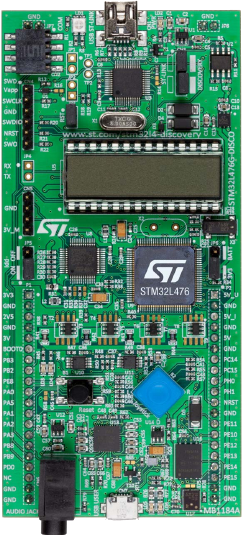
\includegraphics[height=0.3\textheight]{inc/img/discovery}
  \caption{Отладочная плата STM32L476G-Discovery}
  \label{fig:discovery}
\end{figure}

\subsection{Трансивер LoRa}

Модули Semtech LoRa представляют собой ВЧ-трансиверы, с возможностью создания 
топологии M2M (машина-машина) и ``звезда из здвёзд'' (сети LoRa). 
Эти устройства оптимизируют потребление энергии, увеличивая срок службы батарей 
конечных устройств.
Они подробно задокументированы, что делает процесс подключения к интерфейсу
 доступным для широкого круга разработчиков программно-аппаратного обеспечения 
инфраструктуры Интернета вещей.

Серия SX1272/78 имеют бюджет канала в -148 dBm. 
Высокая чувствительность в сочетании с усилителем LNA (малошумящий усилитель)
 +20 дБм обеспечивают надёжную связь для применения в промышленности 
\cite{Rizzi2017}.

\begin{table}[ht]
 \caption{Рабочие частоты для SX1272 и SX1278}
 \begin{tabular}{|c|c|c|}
  \hline
  Устройство & \begin{tabular}[c]{@{}c@{}}Минимальная\\ частота 
  (МГц)\end{tabular} & \begin{tabular}[c]{@{}c@{}}Максимальная\\ частота 
  (МГц)\end{tabular} \\ \hline
  SX1272     & 860                                                               
  & 1020                                                                 \\ 
  \hline
  SX1278     & 137                                                               
  & 525                                                                  \\ 
  \hline
\end{tabular}
 \label{tab:sx127x}
\end{table}

Чувствительность приёмника определяет минимальное значение мощности, которое 
требуется ему для демодуляции и декодирования с целью достижения определенной 
скорости передачи данных. 
Чувствительность обычно выражается в дБм и чем ниже значение, тем лучшую 
чувствительность имеет приёмник, поэтому исходя из таблицы 
\ref{tab:sx127xParams} можно сделать вывод, что SX1278 имеет большую 
чувствительность приёмника перед SX1272.

\begin{table}[ht]
 \caption{Основные параметры приёмопередатчиков LoRa}
 \begin{tabular}{|c|c|c|c|c|}
\hline
\multirow{2}{*}{\begin{tabular}[c]{@{}c@{}}Приёмо-\\ передатчик\end{tabular}} & 
\multicolumn{4}{c|}{Параметры LoRa}                                              
                                                                                 
                                                                                 
                                                          \\ \cline{2-5} 
                                                                              & 
\begin{tabular}[c]{@{}c@{}}SF \\ диапазон\end{tabular} & 
\begin{tabular}[c]{@{}c@{}}Ширина\\  полосы\\ частот (КГц)\end{tabular} & 
\begin{tabular}[c]{@{}c@{}}Эффективная \\ скорость\\ передачи \\ данных\\ 
(кбит/с)\end{tabular} & \begin{tabular}[c]{@{}c@{}}Чувстви-\\ тельность\\ 
(дБм)\end{tabular} \\ \hline
SX1272                                                                        & 
6..12                                                  & от 125 до 500           
                                                & 0,24..37,5                     
                                                                 & -117..-137    
                                                          \\ \hline
SX1278                                                                        & 
6..12                                                  & от 7,8 до 500           
                                                & 0,018..37,5                    
                                                                 & -111..-148    
                                                          \\ \hline
\end{tabular}
 \label{tab:sx127xParams}
\end{table}

Был выбран приёмопередатчик Semtech SX1278. Выбор был обусловлен тем, что он 
уже имелся в наличии и его внутренняя структура схожа с трансивером SX1272 (они 
имеют общее руководство по эксплуатации).
Данный трансивер будет пригоден для исследовательских работ, но следует иметь в 
виду что для коммерческого использования в России следует выбрать трансивер 
SX1272, поскольку частоты около 868 МГц находятся в пределах поддерживаемых 
частот данного трансивера.

\begin{figure}[!h]
  \centering
  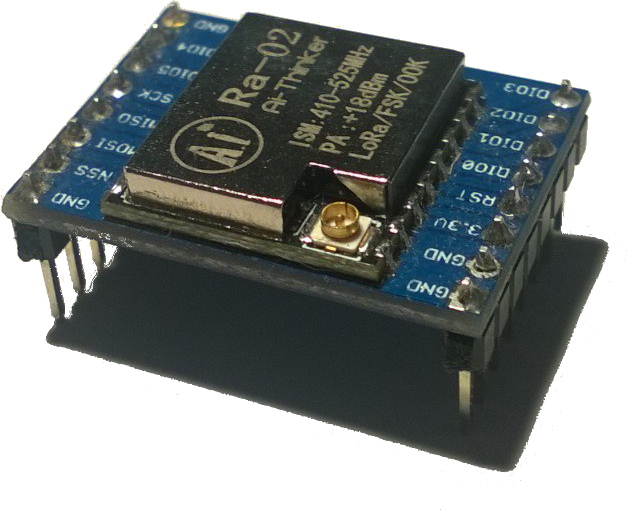
\includegraphics[height=0.3\textheight]{inc/img/SX1278}
  \caption{Трансивер SX1278}
  \label{fig:sx1278}
\end{figure}

Внутренние регистры трансиверов доступны через интерфейс связи SPI.
SPI ""--- это синхронный последовательный полнодуплексный протокол передачи 
данных. 
Обмен по протоколу SPI осуществляют ведущее (\textit{Master}) и подчинённое 
(\textit{Slave}) устройство, приём передачу данных инициирует именно ведущее.

Этот протокол использует 4 линии для связи, которые описываются как:
\begin{itemize}
 \item \textbf{SCLK}. Соответствует тактовому сигналу, генерируется ведущим и 
синхронизирует передачу данных;
 \item \textbf{MOSI} (\textit{Master Out Slave In}). Передача основных данных 
от ведущего к подчиненному устройству;
 \item \textbf{MISO} (\textit{Master In Slave Out}). Передача основных данных 
от подчиненного к ведущему устройству устройству;
 \item $\overline{\text{\textbf{NSS}}}$ (\textit{Slave Select}). Выборка 
%подчиненного устройства. Используется для связи нескольких подчиненных 
%устройств к ведущему. 
\end{itemize}

Радиомодули LoRa работают как подчиненные устройства, а микроконтроллер 
встраиваемой системы будет ведущим в интерфейсе SPI.

На логическом уровне синхронизации и передачи данных для связи SPI требуется 
конфигурация полярности тактирующего сигнала (CPOL) и бит фазы синхронизации 
(CPHA).

Приёмопередатчики LoRa SX1272/78 используют параметры CPOL = 0 и CPHA = 0.
Самый старший бит (MSB) отправленного байта должен быть первым, а скорость SCLK 
не должна превышать 10 МГц.

% Предлагаемая схема соединения здесь?

\section{Описание используемого программного обеспечения}

\subsection{Важность свободного программного обеспечения}

Свободное программное обеспечение играет важную роль для сотрудничества и 
развития поскольку оно обеспечивает технологический суверенитет,
способствует национальным инновациям, оптимизирует расходы на создание 
собственного программного обеспечение, ускоряет местное развитие и 
способствует цифровой интеграции. 

Использование открытого программного обеспечения позволит инфраструктуре 
Интернета вещей:

\begin{itemize}
 \item приобрести технологическую автономию: доступ к исходному коду позволит 
многим пользователям перейти от потребителей к разработчикам программного 
обеспечения;
 \item провести стандартизацию и интеграцию: свободное программное обеспечение 
создается с использованием спецификаций и бесплатных общедоступных 
технологических стандартов, также называемыми ``открытыми стандартами''. Это 
приносит пользу интеграции систем и обмену информацией, гарантирует 
 доступ без ограничений для всех пользователей;
 \item обрести безопасность. Публикация исходных текстов программ или 
приложений способствует их безопасности. Используя открытое программное 
обеспечение, можно узнать и проанализировать, что фактически выполняется 
программой, тип информации, который она обрабатывает и как ей управлять. Хорошая 
безопасность должна основываться на прозрачности. Проприетарное программное 
обеспечение скрывает эти аспекты, и часто неизвестно, сохраняется ли 
конфиденциальность отправляемой информации;
 \item приобрести независимых поставщиков программно-аппаратного обеспечения: 
использование проприетарного программного обеспечения создает зависимость от 
производителя. Как только такое программное обеспечение будет установлено, оно 
будет зависеть от получения обновлений. Во многих случая производитель будет 
принуждать к обновлению до новых версии, даже если это нежелательно.
 \item добиться демократизации информации: информационные технологии заняли 
существенное положение в обществе. Хотя все больше и больше пользователей 
обращаются к указанным технологиям, ``технологический разрыв'' по-прежнему велик 
и является ещё одним фактором социальной изоляции;
 \item добиться экономичности: покупка проприетарного ПО, особенно когда 
производитель имеет монополию на данный вид программного продукта и 
используемых в нём алгоритмов, стоит несравненно больше, чем приобретение и 
использование программного продукта на основе отрытого программного 
обеспечения;
\end{itemize}

\subsection{Основа проекта}

За основу для разработки ПО для микроконтроллера STM32L476VGT6 в связке с 
трансивером SX1278 был взят общедоступный проект от разработчиков альянса LoRa 
Alliance, находящийся по адресу \url{https://github.com/Lora-net/LoRaMac-node} 
(дата обращения 05.06.2018).

%Зачем взял LoRaMac на гитхабе
%Возможно немного слов про открытое ПО
%Ещё чуть чуть про инструменты

\subsection{CMake}

Раздел в процессе написания...

\subsection{HAL}

Раздел в процессе написания...

\subsection{Выбор компилятора для STM32}

Раздел в процессе написания...

\subsection{ST-LINK и Openocd}

Раздел в процессе написания...

\begin{figure}[!h]
  \centering
  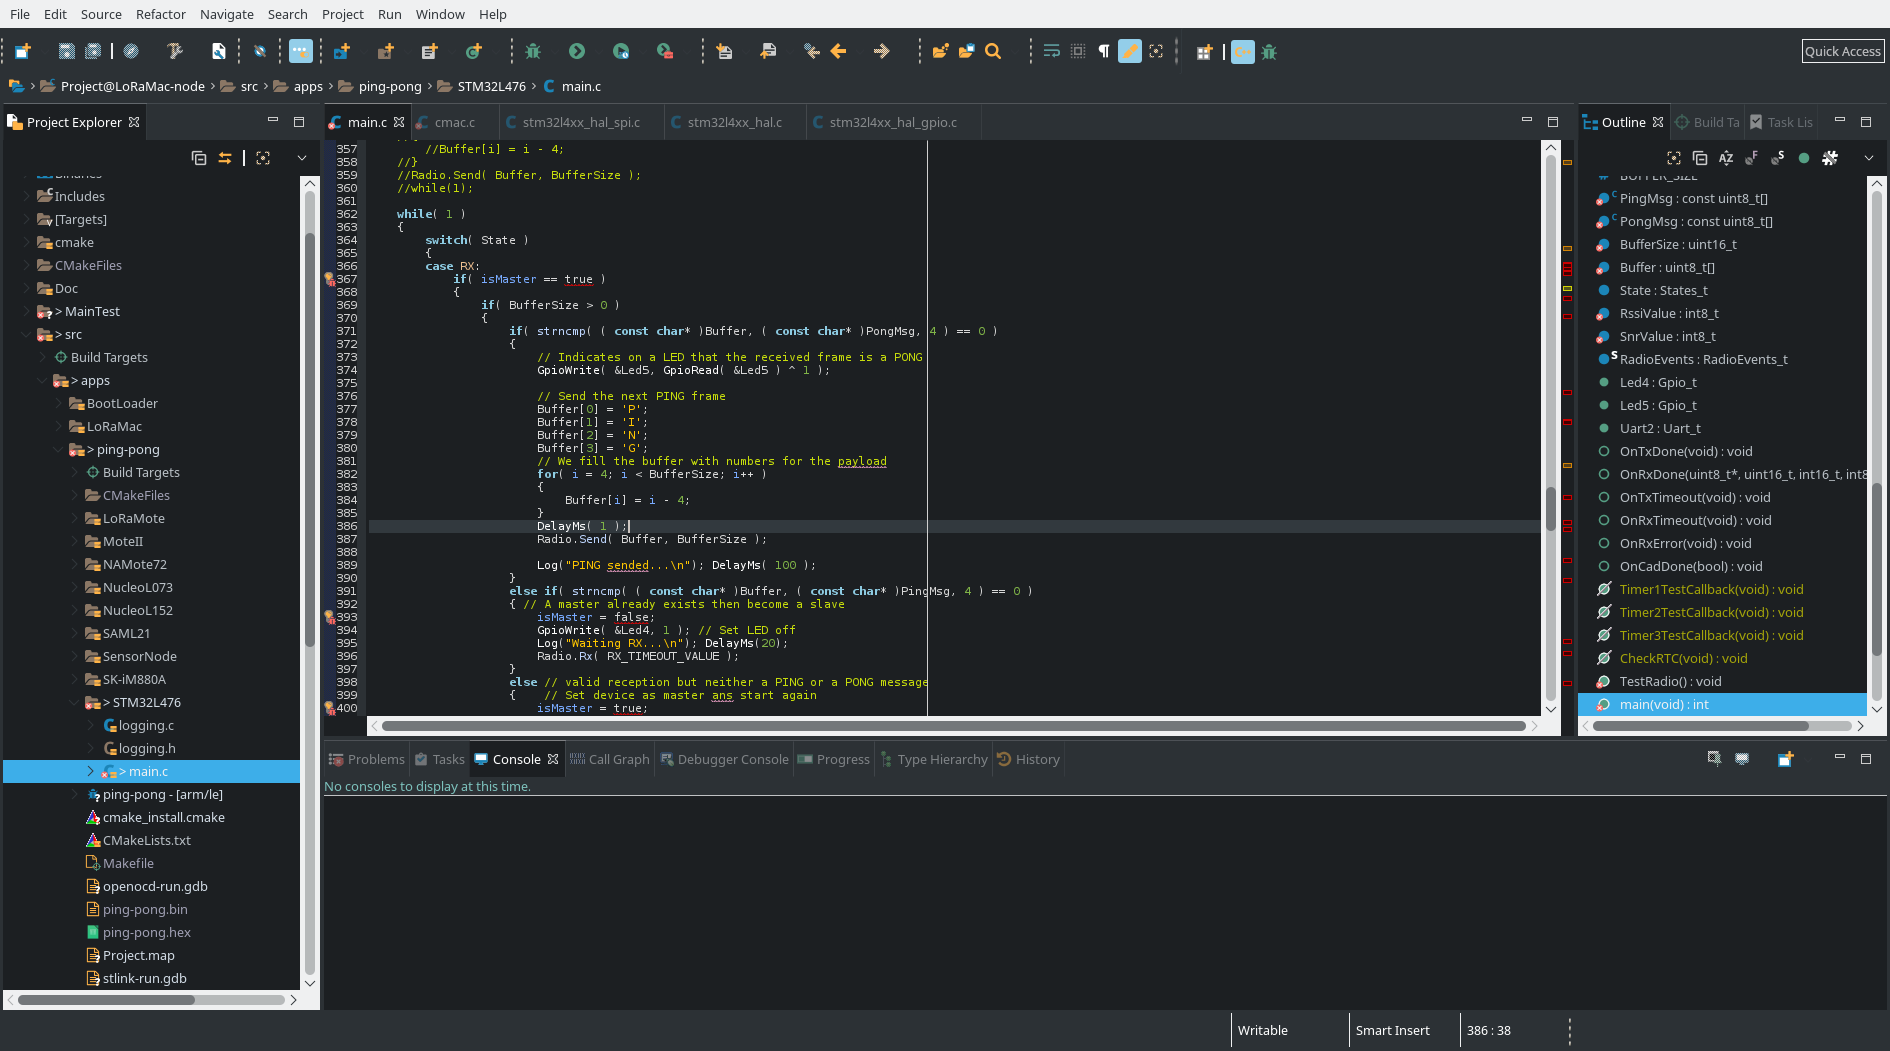
\includegraphics[width=\textwidth]{inc/img/EclipseSTM}
  \caption{Интегрированная среда разработки CDT Eclipse}
  \label{fig:ideeclipse}
\end{figure}


\begin{listing}[H]
 
\end{listing}
\label{lst:boardinit}

\subsection{Структура проекта LoRaMac}
%Правила переноса кода
\begin{figure}[!h]
  \centering
  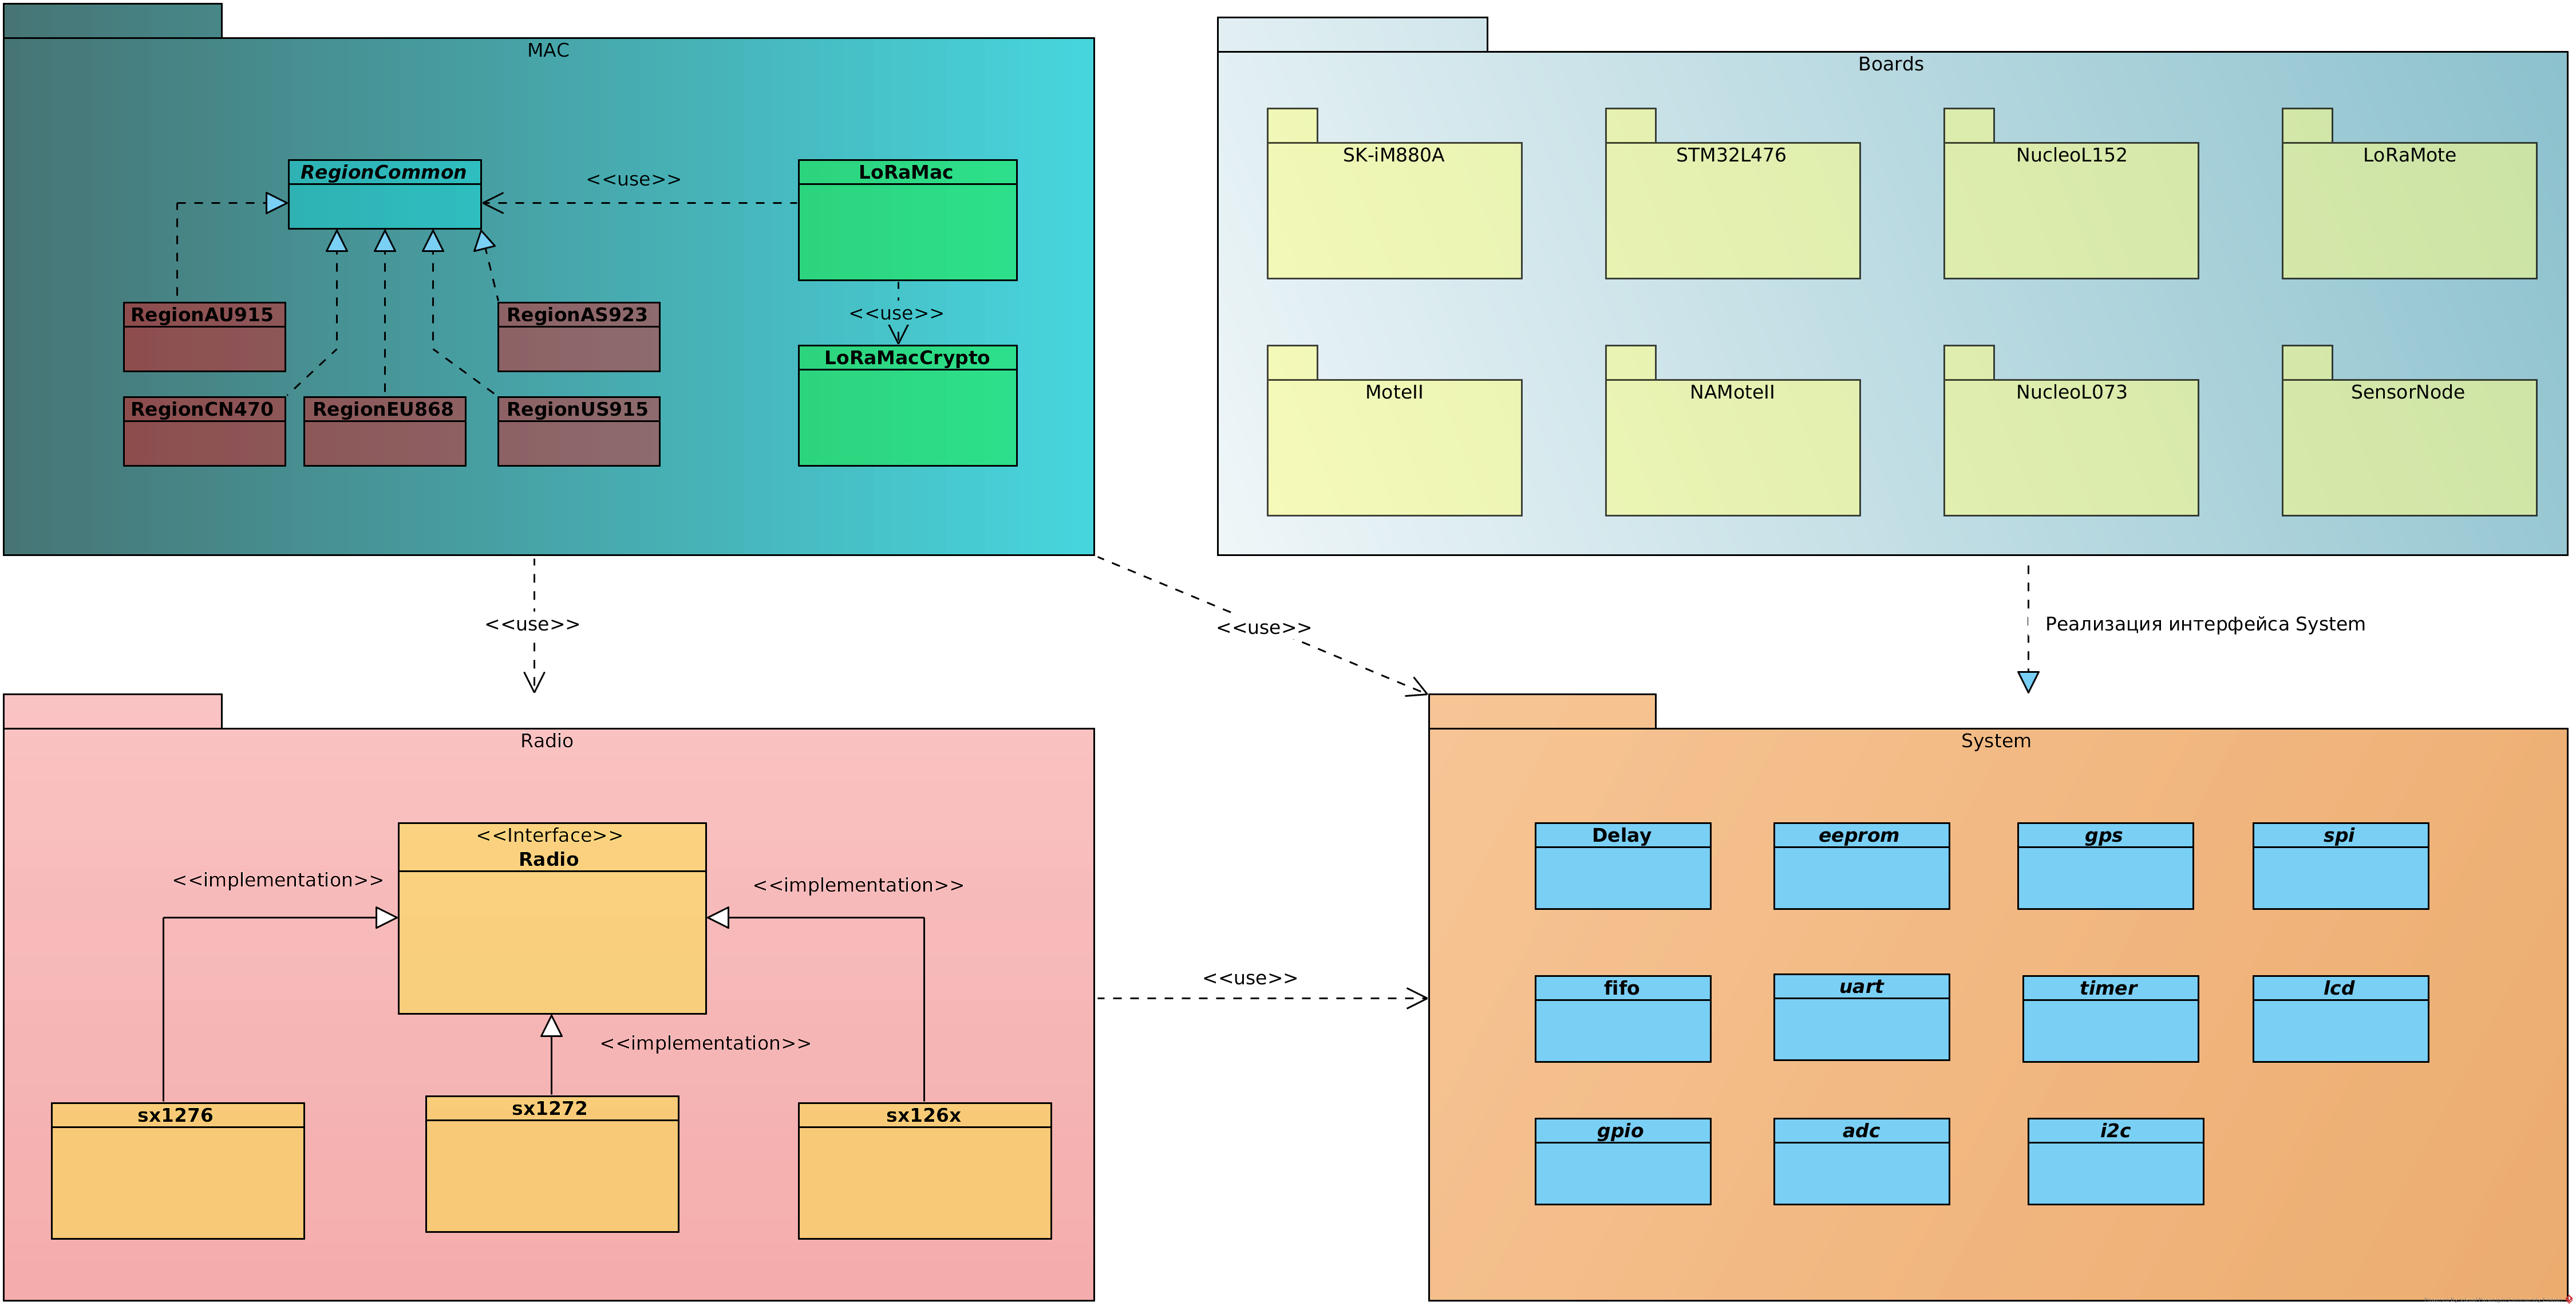
\includegraphics[width=\textwidth]{inc/img/LoRaMacProj}
  \caption{Упрощенная структура проекта LoRaMAC в нотации UML}
  \label{fig:loramacstructure}
\end{figure}

\begin{listing}[H]
% firstline, lastline - какие строки показывать 
\cmakefile{inc/src/CMakeLists.txt}
\caption{Основной CMakeLists} 
\end{listing}
\label{lst:maincmake}

\section{Реализация проекта}

Раздел в процессе написания...

\subsection{Подключение STM32 к трансиверам LoRa}
Раздел в процессе написания...

% Желательно схему

\subsection{Трудности переноса}
Раздел в процессе написания...

% Вспомни про несовместимость HAL и LoRaMac

\subsection{Компиляция и отладка}
Раздел в процессе написания...

%\begin{listing}[H]
% firstline, lastline - какие строки показывать 
%\cfile{inc/src/test.c}
%\caption{Пример — test.c} 
%\end{listing}
%\label{lst:c}

%Можно также использовать окружение \Code{verbatim}, если \Code{listings} чем-то не
%устраивает. Только следует помнить, что табы в нём <<съедаются>>. Существует так же команда \Code{\textbackslash{}verbatiminput} для вставки файла.

%\begin{verbatim}
%a_b = a + b; // русский комментарий
%if (a_b > 0)
    %a_b = 0;
%\end{verbatim}

%%% Local Variables:
%%% mode: latex
%%% TeX-master: "rpz"
%%% End:
